\documentclass[tikz]{standalone}
\usetikzlibrary{backgrounds}
\colorlet{blue}{cyan}
\tikzset{
  inverted/.style = {
    color=white,
    background rectangle/.style={fill},
    show background rectangle
  }
}
\usepackage{tikz}

\begin{document}
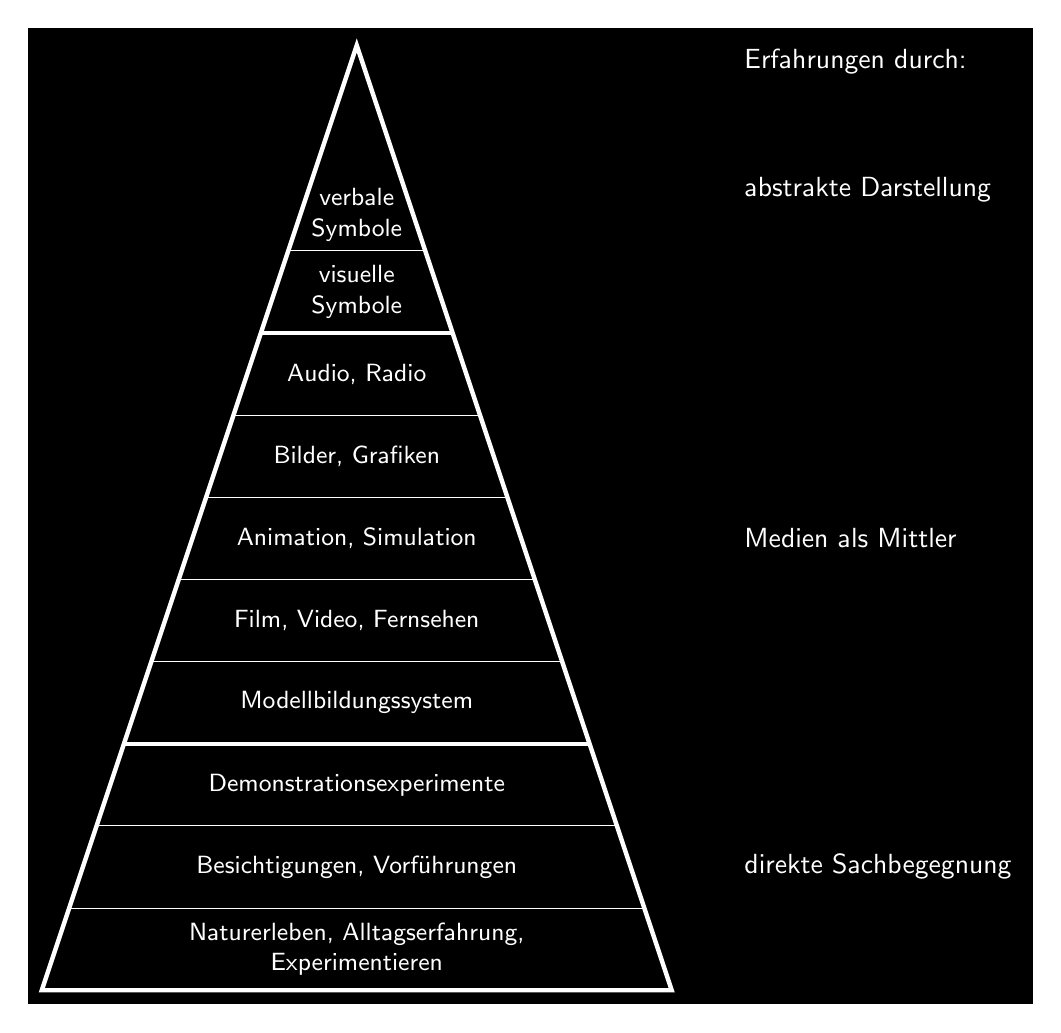
\begin{tikzpicture}[inverted,font=\sffamily]
\pgfmathsetmacro{\H}{12}          % total height
\pgfmathsetmacro{\A}{4}           % half width of base
\pgfmathsetmacro{\TopFactor}{2.5} % factor to increase top level

% level height
\pgfmathsetmacro{\u}{\H/(9+\TopFactor)}

% horizontal line at height y
\newcommand{\hlineat}[2][]{%
  \pgfmathsetmacro{\y}{#2}%
  \pgfmathsetmacro{\x}{\A*(1-\y/\H)}%
  \draw[#1] (-\x,\y) -- (\x,\y);%
}

% outer lines
\coordinate (L) at (-\A,0);
\coordinate (R) at ( \A,0);
\coordinate (T) at (0,\H);
\draw[ultra thick] (L) -- (R) -- (T) -- cycle;

% inner lines
\foreach \k in {1,...,9}{
  \pgfmathsetmacro{\y}{\k*\u}
  \ifnum\k=3
    \hlineat[ultra thick]{\y}
  \else\ifnum\k=8
    \hlineat[ultra thick]{\y}
  \else
    \hlineat[thin]{\y}
  \fi\fi
}

% label between y_low und y_high
\newcommand{\layerlabelY}[3]{%
  \pgfmathsetmacro{\yy}{(#1+#2)/2}%
  \node[align=center,font=\sffamily\small] at (0,\yy) {#3};%
}

% level labels
\layerlabelY{0}{1*\u}{Naturerleben, Alltagserfahrung,\\ Experimentieren}
\layerlabelY{1*\u}{2*\u}{Besichtigungen, Vorführungen}
\layerlabelY{2*\u}{3*\u}{Demonstrationsexperimente}

\layerlabelY{3*\u}{4*\u}{Modellbildungssystem}
\layerlabelY{4*\u}{5*\u}{Film, Video, Fernsehen}
\layerlabelY{5*\u}{6*\u}{Animation, Simulation}
\layerlabelY{6*\u}{7*\u}{Bilder, Grafiken}
\layerlabelY{7*\u}{8*\u}{Audio, Radio}

\layerlabelY{8*\u}{9*\u}{visuelle\\ Symbole}
%\layerlabelY{9*\u}{\H}{verbale\\ Symbole}
\node[align=center,anchor=south,font=\sffamily\small] at (0,9*\u) {verbale\\ Symbole};

% additional labels
\node[anchor=west] at (\A+0.8,\H-0.2) {Erfahrungen durch:};

\pgfmathsetmacro{\yabs}{(8*\u+\H)/2}     % top two levels
\pgfmathsetmacro{\ymed}{(3*\u+8*\u)/2}   % center 5 levels
\pgfmathsetmacro{\ydir}{(0+3*\u)/2}      % lower 3 levels

\node[anchor=west] at (\A+0.8,\yabs) {abstrakte Darstellung};
\node[anchor=west] at (\A+0.8,\ymed) {Medien als Mittler};
\node[anchor=west] at (\A+0.8,\ydir) {direkte Sachbegegnung};
\end{tikzpicture}
\end{document}
